\documentclass[11pt]{article}
\usepackage[a4paper,margin=0.65in]{geometry}
\usepackage[T1]{fontenc}
\usepackage{amsmath,amssymb,amsfonts}
\usepackage{graphicx}
\usepackage{tikz}
\usepackage{pdfpages}
\usepackage[english,shorthands=off]{babel}
\usepackage{fancyhdr}
\usepackage[bookmarks=false,colorlinks=false]{hyperref}
\usepackage[protrusion=true,expansion=false]{microtype}
\emergencystretch=3em
\tolerance=600
\providecommand{\modd}{\mathrm{mod}}
\providecommand{\Disc}{\mathrm{Disc}}
\providecommand{\canont}{}
\providecommand{\asterism}{*}
\providecommand{\Hessian}{H}
\providecommand{\tome}{}
\providecommand{\page}{p.}
\providecommand{\elqr}{\operatorname{elqr}}
\providecommand{\elta}{\operatorname{elta}}
\pagestyle{fancy}\fancyhf{}\fancyhead[L]{Pages 301--325}\fancyhead[R]{Cayley --- Collected Papers, Vol. III}\renewcommand{\headrulewidth}{0.4pt}
\setlength{\headheight}{15pt}

\begin{document}

\begin{center}
{\Large\bfseries Cayley --- Collected Mathematical Papers, Vol.\ III}\\[0.5em]
{\large PDF pages 301--325 (printed pp.~279--303)}\\[0.5em]
{\small Papers 212 (conclusion) and 213 (opening)}
\end{center}

\bigskip

%=================================================================
% PAPER 212 (continued) --- printed pp. 279--292 (PDF pp. 301--314)
%=================================================================

\section*{212. A Memoir on the Problem of Disturbed Elliptic Motion \textit{(continued)}}

\medskip
\noindent[PDF p.~301; printed p.~279.] sun's orbit from a departure-point, defined as above, in that orbit), and the position of the planet would then be determined by means of the longitude, latitude, and radius vector. The term \emph{sidereal longitude} is, I think, used in Physical Astronomy rather loosely to denote the longitude in the mean ecliptic from the mean equinox, less the precession; so defined it is not practically different from, and may I think in all cases be replaced by the longitude as measured from a departure-point in the mean ecliptic.

\medskip
\noindent Returning from this digression, the assumed equation, $d\varpi=\cos\phi\,d\theta$, gives the expression for the variation $d\varpi$ of the departure of the node, and we now have in the place of the former six equations the seven equations
\[
dr = 0,
\]
\[
d\,\mathfrak{p} = 0,
\]
\[
d\frac{nae\sin f}{\sqrt{1-e^{2}}} = \frac{d\Omega}{dr}\,dt,
\]
\[
d\,na^{2}\sqrt{1-e^{2}} = \frac{d\Omega}{d\mathfrak{z}}\,dt,
\]
\[
d\phi = \frac{\cot\mathfrak{z}}{na^{2}\sqrt{1-e^{2}}}\,\frac{d\Omega}{d\phi}\,dt,
\]
\[
d\varpi = \frac{-\cot\phi}{na^{2}\sqrt{1-e^{2}}}\,\frac{d\Omega}{d\phi}\,dt,
\]
\[
d\theta = \frac{\operatorname{cosec}\phi}{na^{2}\sqrt{1-e^{2}}}\,\frac{d\Omega}{d\phi}\,dt,
\]
where as before $\Omega=\Omega(r,\mathfrak{p},\sigma,\theta,\phi)$.

\medskip
\noindent But the value of $\mathfrak{z}$ is $\mathfrak{z}=\mathfrak{p}-\sigma$, and $\Omega$ can be expressed, and that in a single way only, viz.\ by means of the substitution of $\mathfrak{p}-\sigma$ in the place of $\mathfrak{z}$, in the form $\Omega = \Omega(r,\mathfrak{p},\sigma,\theta,\phi)$, and if on the right-hand side $\Omega=\Omega(r,\mathfrak{p},\mathfrak{z},\theta,\phi)$ as before, then we have
\[
\frac{d\Omega}{dr} = \frac{d\Omega}{dr},
\]
\[
\frac{d\Omega}{d\mathfrak{p}} = \frac{d\Omega}{d\mathfrak{z}},
\]
\[
\frac{d\Omega}{d\sigma} = -\frac{d\Omega}{d\mathfrak{z}},
\]
\[
\frac{d\Omega}{d\phi} = \frac{d\Omega}{d\phi},
\]
\[
\frac{d\Omega}{d\theta} = \frac{d\Omega}{d\theta},
\]

\bigskip
\noindent[PDF p.~302; printed p.~280.] where on the left-hand side $\Omega = \Omega(r,\mathfrak{p},\sigma,\theta,\phi)$. The function $\Omega$ so expressed satisfies, of course, the partial differential equation
\[
\frac{d\Omega}{d\mathfrak{p}} + \frac{d\Omega}{d\sigma} = 0
\]
(which conversely implies that $\mathfrak{p}$, $\sigma$ only enters through the function $\mathfrak{p}-\sigma$), and it also satisfies the partial differential equation obtained from the before-mentioned equation
\[
\cot\mathfrak{z}\,\frac{d\Omega}{d\phi} = \cot\phi\,\frac{d\Omega}{d\sigma} - \operatorname{cosec}\phi\,\frac{d\Omega}{d\theta}, \qquad (\Omega=\Omega(r,\mathfrak{z},\theta,\phi)),
\]
by the introduction of the transformed expressions of the differential coefficients, and which may be written
\[
\cot\mathfrak{z}\,\frac{d\Omega}{d\phi} = \cot\phi\,\frac{d\Omega}{d\sigma} - \operatorname{cosec}\phi\,\frac{d\Omega}{d\theta},
\]
where $\Omega = \Omega(r,\mathfrak{p},\sigma,\theta,\phi)$.

\medskip
\noindent Using the last-mentioned equation to transform the value of $d\phi$, the expressions for the variations become
\[
dr=0,\qquad d\mathfrak{p}=0,
\]
\[
d\frac{nae\sin f}{\sqrt{1-e^{2}}} = \frac{d\Omega}{dr}\,dt,
\]
\[
d\,na^{2}\sqrt{1-e^{2}} = \frac{d\Omega}{d\mathfrak{p}}\,dt,
\]
\[
d\phi = \frac{-\cot\phi}{na^{2}\sqrt{1-e^{2}}}\,\frac{d\Omega}{d\sigma}\,dt - \frac{\operatorname{cosec}\phi}{na^{2}\sqrt{1-e^{2}}}\,\frac{d\Omega}{d\theta}\,dt,
\]
\[
d\sigma = \frac{-\cot\phi}{na^{2}\sqrt{1-e^{2}}}\,\frac{d\Omega}{d\phi}\,dt,
\]
\[
d\theta = \frac{\operatorname{cosec}\phi}{na^{2}\sqrt{1-e^{2}}}\,\frac{d\Omega}{d\phi}\,dt,
\]
where $\Omega = \Omega(r,\mathfrak{p},\sigma,\theta,\phi)$ as before.

\medskip
\noindent I suppose now that the orbit of the planet, instead of being referred to a fixed plane, is referred to a moveable plane or orbit of reference. It is assumed that the longitudes in the orbit of reference are measured from a departure-point defined as above,---that is, from the point in which the orbit of reference is intersected by any orthogonal trajectory of the successive positions of the orbit of reference. And the

\bigskip
\noindent[PDF p.~303; printed p.~281.] position in regard to the fixed plane, of the orbit of reference, and of the departure-point in this orbit, are determined by $\theta'$, $\sigma'$, $\phi'$, ---that is, we have for the orbit of reference,
\begin{itemize}
\item[] $\theta'$, the longitude of node,
\item[] $\sigma'$, the departure of node,
\item[] $\phi'$, the inclination.
\end{itemize}

\noindent The position of the planet's orbit in relation to the moveable orbit of reference is determined in like manner by $\Theta$, $\Sigma$, $\Phi$,---that is, we have for the planet's orbit in relation to the orbit of reference,
\begin{itemize}
\item[] $\Theta$, the longitude of node,
\item[] $\Sigma$, the departure of node,
\item[] $\Phi$, the inclination.
\end{itemize}

\noindent Hence if, as before, $\theta$, $\sigma$, $\phi$, belong to the orbit of the planet considered in relation to the fixed plane, $\Sigma-\sigma$, $\Theta-\sigma'$, $\theta-\theta'$, will be the sides of a spherical triangle, the opposite angles of which are $\phi'$, $180^{\circ}-\phi$ and $\Phi$.

\medskip
\[
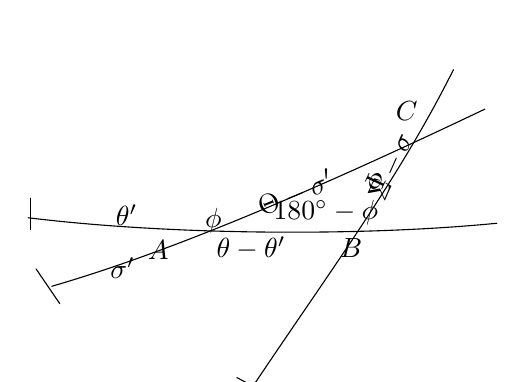
\begin{tikzpicture}[scale=1.0,line cap=round,line join=round]
  \coordinate (A) at (0,0);
  \coordinate (B) at (2.45,0.03);
  \coordinate (C) at (3.42,1.28);
  \draw (-1.65,0.17) .. controls (0.15,-0.05) and (2.55,-0.07) .. (4.30,0.10);
  \draw (-1.35,-0.70) .. controls (0.20,-0.25) and (2.05,0.55) .. (4.15,1.55);
  \draw (1.15,-2.05) .. controls (2.15,-0.55) and (3.05,0.65) .. (3.75,2.05);
  \draw (-1.55,-0.48) -- (-1.25,-0.92);
  \draw (-1.62,0.02) -- (-1.62,0.42);
  \draw (1.00,-1.86) -- (1.42,-2.08);
  \node[below] at (A) {$A$};
  \node[below] at (B) {$B$};
  \node[above left] at (C) {$C$};
  \node at (-0.40,0.20) {$\theta'$};
  \node at (-0.45,-0.47) {$\sigma'$};
  \node at (1.18,-0.22) {$\theta-\theta'$};
  \node[rotate=22] at (1.75,0.48) {$\Theta-\sigma'$};
  \node[rotate=66] at (2.96,0.82) {$\Sigma-\sigma$};
  \node at (0.70,0.13) {$\phi$};
  \node at (2.13,0.23) {$180^{\circ}-\phi$};
  \node[rotate=65] at (2.76,0.63) {$\Phi$};
\end{tikzpicture}
\]

\medskip
\noindent Putting for shortness $S=\Sigma-\sigma$, $S'=\Theta-\sigma'$, $G=\theta-\theta'$, so that these symbols denote
\begin{itemize}
\item[] $S$, the distance of node, along planet's orbit, from fixed plane,
\item[] $S'$, the distance of node, along orbit of reference, from fixed plane,
\item[] $G$, the distance in fixed plane of the nodes on fixed plane,
\end{itemize}
the sides of the spherical triangle are $S$, $S'$, $G$, and the opposite angles are $\phi'$, $180^{\circ}-\phi$, $\Phi$.

\bigskip
\noindent[PDF p.~304; printed p.~282.] Calling the sides $A$, $B$, $C$, and the opposite angles $a$, $b$, $c$, the general formul\ae{} for a spherical triangle give without difficulty,
\[
dC = -\cos b\,dA - \cos a\,dB + \frac{\sin A\sin B\sin c}{\sin C}\,dc,
\]
\[
da = \frac{\cos C\sin a}{\sin C}\,dA + \frac{\sin A\cos b}{\sin C}\,dB + \frac{\sin A\sin c}{\sin C}\,dc \cdot \frac{1}{\sin C},
\]
\[
db = \frac{\cos C\sin b}{\sin C}\,dA + \frac{\sin A}{\sin C}\,dB + \frac{\sin B\cos a}{\sin C}\,dc,
\]
and conversely
\[
dc = -\cos B\,da - \cos A\,db + \frac{\sin a\sin b\sin C}{\sin c}\,dC,
\]
\[
dA = \frac{\sin B}{\sin c}\,da - \frac{\cos c\sin A}{\sin c}\,db - \frac{\sin a\cos B}{\sin c}\,dC,
\]
\[
dB = -\frac{\cos c\sin B}{\sin c}\,da + \frac{\sin A}{\sin c}\,db - \frac{\sin b\cos A}{\sin c}\,dC,
\]
which, in the present case, become
\[
d\Phi = -\cos S\,d\phi' - \cos S'\,d\phi + \frac{\sin\phi'\sin\phi\sin G}{\sin\Phi}\,dG,
\]
\[
dS = -\frac{\sin\phi'\sin S}{\sin\Phi}\,d\phi' + \frac{\cos\Phi\cos S}{\sin\Phi}\,dS' + \frac{\sin\phi'\sin G}{\sin\Phi}\,dG,
\]
\[
dS' = -\frac{\cos\Phi\sin S'}{\sin\Phi}\,d\phi' + \frac{\sin\phi}{\sin\Phi}\,dS' + \frac{\sin\phi'\sin G}{\sin\Phi}\,dG,
\]
and
\[
dG = -\cos S'\,d\phi' - \cos\phi\,dS + \frac{\sin S\sin S'\sin\Phi}{\sin G}\,d\Phi,
\]
\[
d\phi = -\frac{\sin\phi'}{\sin G}\,dS' + \frac{\cos G\sin\phi}{\sin G}\,dS + \frac{\sin S\cos\phi'}{\sin G}\,d\Phi,
\]
\[
d\phi' = -\frac{\cos G\sin\phi'}{\sin G}\,dS' + \frac{\sin S}{\sin G}\,dS + \frac{\sin S\cos\phi}{\sin G}\,d\Phi,
\]
and we have also
\[
dS = d\Sigma - d\sigma,
\]
\[
dS' = d\Theta - d\sigma',
\]
\[
dG = d\theta - d\theta'.
\]

\medskip
\noindent Hence, observing that $\sin S\sin\phi = \sin S'\sin\phi'$, the preceding equations may be written
\begin{align*}
d\Phi &= -\cos S\,d\phi' - \cos S'\,d\phi + \sin S\sin\phi\,dG - \sin S'\sin\phi'\,dG, \\
d\Sigma &= d\sigma - \operatorname{cosec}\Phi\sin S\,d\phi' + \cot\Phi\sin S\,d\phi + \operatorname{cosec}\Phi\sin\phi\cos S(dG - d\theta'), \\
d\Theta &= d\sigma' - \cot\Phi\sin S\,d\phi' + \operatorname{cosec}\Phi\sin S\,d\phi + \operatorname{cosec}\Phi\sin\phi\cos S(dG - d\theta'),
\end{align*}

\bigskip
\noindent[PDF p.~305; printed p.~283.] and
\begin{align*}
d\theta &= d\theta' + \cos\phi'(d\Theta - d\sigma') - \cos\phi(d\Sigma - d\sigma) + \sin S\sin\phi\,d\Phi, \\
d\phi &= \operatorname{cosec} G\sin\phi'(d\Theta - d\sigma') + \cot G\sin\phi(d\Sigma - d\sigma) + \operatorname{cosec} G\sin S\cos\phi'\,d\Phi, \\
d\phi' &= -\cot G\sin\phi'(d\Theta - d\sigma') + \operatorname{cosec} G\sin\phi(d\Sigma - d\sigma) + \operatorname{cosec} G\sin S\cos\phi\,d\Phi,
\end{align*}
and it is proper to remark, that in obtaining these equations no use has been made of the equations $d\sigma=\cos\phi\,d\theta$, $d\sigma' = \cos\phi'\,d\theta'$.

\medskip
\noindent The term in $d\Theta$ which contains $d\sigma'$, \&c.\ may be written
\[
(d\sigma' - \cos\phi'\,d\theta') + \cos\phi'\,d\theta' + \cot\phi'\sin S\,d\phi' - \operatorname{cosec}\phi'\sin\phi\cos S\,d\theta',
\]
which is equal to
\[
(d\sigma' - \cos\phi'\,d\theta') + \cot\phi'(\sin S\,d\phi' - \cos S\sin\phi\,d\theta');
\]
and the term in $d\Sigma$ which contains $d\sigma$, \&c.\ may be written
\[
(d\sigma - \cos\phi\,d\theta) + \cos\phi\,d\theta - \cot\phi\sin S\,d\phi + \operatorname{cosec}\phi\sin\phi'\cos S\,d\theta,
\]
which is equal to
\[
(d\sigma - \cos\phi\,d\theta) - \cot\phi(\sin S\,d\phi - \cos S\sin\phi'\,d\theta);
\]
reductions which depend on
\[
\cos\phi'\operatorname{cosec}\phi\sin\phi'\cos S = \cot\phi'\sin\phi'\cos S',
\]
\[
\cos\phi + \operatorname{cosec}\phi'\sin\phi\cos S = \cot\phi'\sin\phi'\cos S,
\]
or, what is the same thing,
\[
\cos\phi\sin\Phi\sin\phi'\cos\Phi\cos S = \sin\phi\cos S',
\]
\[
\cos\phi'\sin\Phi\sin\phi\cos\Phi\cos S = \sin\phi'\cos S,
\]
which are relations between the sides and angles of the spherical triangle. And we then have
\begin{align*}
d\Phi &= (\cos S\,d\phi' + \sin S\sin\phi\,d\theta') - (\cos S'\,d\phi + \sin S'\sin\phi'\,d\theta'), \\
d\Theta &= (d\sigma' - \cos\phi'\,d\theta') - \operatorname{cosec}\Phi(\sin S\,d\phi - \cos\phi\sin\phi'\,d\theta) + \cot\phi'(\sin S\,d\phi' - \cos S\sin\phi\,d\theta'), \\
d\Sigma &= (d\sigma - \cos\phi\,d\theta) - \cot\Phi(\sin S\,d\phi - \cos S\sin\phi\,d\theta) + \operatorname{cosec}\Phi(\sin S\,d\phi' - \cos S\sin\phi'\,d\theta'),
\end{align*}
expressions which may be simplified by omitting the terms $(d\sigma' - \cos\phi'\,d\theta')$ and $(d\sigma - \cos\phi\,d\theta)$.

\medskip
\noindent Next substituting for $d\sigma$, $d\phi$, $d\theta$, their values, we obtain,
\[
dr = 0,\qquad d\mathfrak{p}=0,
\]
\[
d\frac{nae\sin f}{\sqrt{1-e^{2}}} = \frac{d\Omega}{dr}\,dt,
\]

\bigskip
\noindent[PDF p.~306; printed p.~284.]
\[
d\,na^{2}\sqrt{1-e^{2}} = \frac{d\Omega}{d\mathfrak{p}}\,dt,
\]
\[
d\Phi = \frac{1}{na^{2}\sqrt{1-e^{2}}}\left(\sin S'\,\frac{d\Omega}{d\phi} - \cos S\Bigl(\cot\phi\,\frac{d\Omega}{d\sigma} + \operatorname{cosec}\phi\,\frac{d\Omega}{d\theta}\Bigr)\right)dt - (\sin S'\,d\phi' + \sin S\sin\phi\,d\theta'),
\]
\[
d\Sigma = \frac{\cot\Phi}{na^{2}\sqrt{1-e^{2}}}\left(\cos S\,\frac{d\Omega}{d\phi} + \sin S\Bigl(\cot\phi\,\frac{d\Omega}{d\sigma} + \operatorname{cosec}\phi\,\frac{d\Omega}{d\theta}\Bigr)\right)dt + \operatorname{cosec}\Phi(\sin S'\,d\phi' - \cos S\sin\phi'\,d\theta'),
\]
\[
d\Theta = \frac{\operatorname{cosec}\Phi}{na^{2}\sqrt{1-e^{2}}}\left(\cos S\,\frac{d\Omega}{d\phi} + \sin S\Bigl(\cot\phi\,\frac{d\Omega}{d\sigma} + \operatorname{cosec}\phi\,\frac{d\Omega}{d\theta}\Bigr)\right)dt + \cot\Phi(\sin S'\,d\phi' - \cos S\sin\phi'\,d\theta'),
\]
where $\Omega = \Omega(r,\mathfrak{p},\sigma,\theta,\phi)$ as before.

\medskip
\noindent But $\Omega$ may be expressed in the form $\Omega = \Omega(r,\mathfrak{p},\Sigma,\Theta,\Phi)$, or disregarding $\sigma'$, $\theta'$, $\phi'$, in the form $\Omega = \Omega(r,\mathfrak{p},\Sigma,\Theta,\Phi)$, and to effect the transformation of the differential coefficients we must write,
\begin{align*}
d\Phi &= \cos S\,d\phi + \sin S\sin\phi\,d\theta, \\
d\Theta &= -\operatorname{cosec}\Phi(\sin S\,d\phi - \cos S\sin\phi\,d\theta), \\
d\Sigma &= (d\sigma - \cos\phi\,d\theta) - \cot\Phi(\sin S\,d\phi - \cos S\sin\phi\,d\theta),
\end{align*}
or, what is the same thing,
\begin{align*}
d\phi &= \cos S\,d\Phi - \sin S\sin\Phi\,d\Theta, \\
d\theta &= -\operatorname{cosec}\phi(\sin S\,d\Phi + \cos S\sin\Phi\,d\Theta), \\
d\sigma &= d\Sigma - \cos\phi\,d\Theta + \cot\phi(\sin S\,d\Phi + \cos S\sin\Phi\,d\Theta),
\end{align*}
and substituting in
\[
\frac{d\Omega}{dr}\,dr + \frac{d\Omega}{d\mathfrak{p}}\,d\mathfrak{p} + \frac{d\Omega}{d\sigma}\,d\sigma + \frac{d\Omega}{d\theta}\,d\theta + \frac{d\Omega}{d\phi}\,d\phi
= \frac{d\Omega}{dr}\,dr + \frac{d\Omega}{d\mathfrak{p}}\,d\mathfrak{p} + \frac{d\Omega}{d\Sigma}\,d\Sigma + \frac{d\Omega}{d\Theta}\,d\Theta + \frac{d\Omega}{d\Phi}\,d\Phi,
\]
if on the right-hand side $\Omega = \Omega(r,\mathfrak{p},\sigma,\theta,\phi)$ as before, then we have
\[
\frac{d\Omega}{dr} = \frac{d\Omega}{dr},\qquad \frac{d\Omega}{d\mathfrak{p}} = \frac{d\Omega}{d\mathfrak{p}},\qquad \frac{d\Omega}{d\Sigma} = \frac{d\Omega}{d\sigma},
\]
\[
\frac{d\Omega}{d\Theta} = -\Bigl(-\cos\phi + \cot\phi\cos S\sin\Phi\Bigr)\frac{d\Omega}{d\sigma} + \operatorname{cosec}\phi\cos S\sin\Phi\,\frac{d\Omega}{d\theta} - \sin S\sin\Phi\,\frac{d\Omega}{d\phi},
\]
\[
\frac{d\Omega}{d\Phi} = \cot\phi\sin S\,\frac{d\Omega}{d\sigma} - \operatorname{cosec}\phi\sin S\,\frac{d\Omega}{d\theta} + \cos S\,\frac{d\Omega}{d\phi},
\]
where on the left-hand side $\Omega = \Omega(r,\mathfrak{p},\Sigma,\Theta,\Phi)$.

\bigskip
\noindent[PDF p.~307; printed p.~285.] The last three equations give
\[
\cos S\,\frac{d\Omega}{d\phi} + \sin S\Bigl(\cot\phi\,\frac{d\Omega}{d\sigma} + \operatorname{cosec}\phi\,\frac{d\Omega}{d\theta}\Bigr) = \frac{d\Omega}{d\Phi},
\]
\[
-\sin S\,\frac{d\Omega}{d\phi} + \cos S\Bigl(\cot\phi\,\frac{d\Omega}{d\sigma} + \operatorname{cosec}\phi\,\frac{d\Omega}{d\theta}\Bigr) = \cot\Phi\,\frac{d\Omega}{d\Sigma} + \operatorname{cosec}\Phi\,\frac{d\Omega}{d\Theta},
\]
and the formul\ae{} for the variations become
\[
dr = 0,\qquad d\mathfrak{p} = 0,
\]
\[
d\frac{nae\sin f}{\sqrt{1-e^{2}}} = \frac{d\Omega}{dr}\,dt,
\]
\[
d\,na^{2}\sqrt{1-e^{2}} = \frac{d\Omega}{d\mathfrak{p}}\,dt,
\]
\[
d\Phi = \frac{-\cot\Phi}{na^{2}\sqrt{1-e^{2}}}\,\frac{d\Omega}{d\Sigma}\,dt - \frac{\operatorname{cosec}\Phi}{na^{2}\sqrt{1-e^{2}}}\,\frac{d\Omega}{d\Theta}\,dt - (\cos S'\,d\phi' + \sin S'\sin\phi'\,d\theta'),
\]
\[
d\Sigma = \frac{\cot\Phi}{na^{2}\sqrt{1-e^{2}}}\,\frac{d\Omega}{d\Phi}\,dt + \operatorname{cosec}\Phi(\sin S'\,d\phi' - \cos S'\sin\phi'\,d\theta'),
\]
\[
d\Theta = \frac{\operatorname{cosec}\Phi}{na^{2}\sqrt{1-e^{2}}}\,\frac{d\Omega}{d\Phi}\,dt + \cot\Phi(\sin S'\,d\phi' - \cos S'\sin\phi'\,d\theta'),
\]
where $\Omega = \Omega(r,\mathfrak{p},\Sigma,\Theta,\Phi)$. It will be recollected that the value of $S'$ is $=\Theta-\sigma'$. It may be noticed that
\[
d\Sigma - \cos\Phi\,d\Theta = \sin\Phi(\sin S'\,d\phi' - \cos S'\sin\phi'\,d\theta').
\]

\medskip
\noindent The system just obtained is, except as regards the terms involving $d\phi'$ and $d\theta'$, precisely similar in its form to that in which the planet is referred to a fixed plane, or where $\Omega = \Omega(r,\mathfrak{p},\sigma,\theta,\phi)$, and this is of course as it should be.

\medskip
\noindent We have now
\[
\mathfrak{p} = \varpi + f,
\]
\[
r = a\,\elqr(e,g),
\]
\[
f = \elta(e,g),
\]
so that the position of the planet is determined by means of the elements $a$, $e$, $g$, $\varpi$, $\Sigma$, $\Theta$, $\Phi$. To find the variations of these elements, substituting for $r$ its value in terms of $f$, the first, third, and fourth equations are
\[
d\,\frac{a(1-e^{2})}{1+e\cos f} = 0,
\]
\[
d\,\frac{nae\sin f}{\sqrt{1-e^{2}}} = \frac{d\Omega}{dr}\,dt,
\]
\[
d\,na^{2}\sqrt{1-e^{2}} = \frac{d\Omega}{d\mathfrak{p}}\,dt,
\]

\bigskip
\noindent[PDF p.~308; printed p.~286.] which give
\[
\frac{e\sin f\,df}{1-e^{2}}\,de - \frac{2e+(1+e^{2})\cos f}{1-e^{2}}\,de + \frac{1+e\cos f}{a}\,da = 0,
\]
\[
e\cos f\,df + \sin f\,de = \frac{\sqrt{1-e^{2}}}{na}\,\frac{d\Omega}{dr}\,dt + \frac{na^{2}\sqrt{1-e^{2}}}{e\sin f}\,\frac{d\Omega}{d\mathfrak{p}}\,dt,
\]
\[
-\,de + \frac{1-e^{2}}{2ne}\,da = \frac{\sqrt{1-e^{2}}}{na^{2}}\,\frac{d\Omega}{d\mathfrak{p}}\,dt,
\]
and we thence obtain
\[
da = \frac{2e\sin f}{n\sqrt{1-e^{2}}}\,\frac{d\Omega}{dr}\,dt + \frac{2(1+e\cos f)^{2}}{na(1-e^{2})}\,\frac{d\Omega}{d\mathfrak{p}}\,dt,
\]
\[
de = \frac{\sqrt{1-e^{2}}\sin f}{na}\,\frac{d\Omega}{dr}\,dt + \frac{e+2\cos f+e\cos^{2}f}{na^{2}\sqrt{1-e^{2}}}\,\frac{d\Omega}{d\mathfrak{p}}\,dt,
\]
\[
df = \frac{n\sqrt{1-e^{2}}\cos f\,d\Omega}{nae}\,dt - \frac{(2+e\cos f)\sin f}{na^{2}e}\,\frac{d\Omega}{d\mathfrak{p}}\,dt,
\]
the last of which equations, combined with
\[
df + \frac{n\sqrt{1-e^{2}}}{(1-e^{2})^{3/2}}\,dg - \frac{na e\sin f\cos f}{(1-e^{2})^{2}}\,de = 0,
\]
gives
\[
dg = \frac{(1-e^{2})(-2e+\cos f + e\cos^{2}f)}{nae(1+e\cos f)^{2}}\,\frac{d\Omega}{dr}\,dt - \frac{(2+e\cos f)\sin f}{na^{2}e}\,\frac{d\Omega}{d\mathfrak{p}}\,dt.
\]

\medskip
\noindent The fourth equation of the formul\ae{} for the variations, viz., $d\phi=0$, gives $0 = d\varpi + df$, and therefore $d\varpi = -df$, that is,
\[
d\varpi = -\frac{\sqrt{1-e^{2}}\cos f}{nae}\,\frac{d\Omega}{dr}\,dt + \frac{(2+e\cos f)\sin f}{na^{2}\sqrt{1-e^{2}}}\,\frac{d\Omega}{d\mathfrak{p}}\,dt,
\]
and the complete system becomes therefore
\[
da = \frac{2e\sin f}{n\sqrt{1-e^{2}}}\,\frac{d\Omega}{dr}\,dt + \frac{2(1+e\cos f)^{2}}{na(1-e^{2})}\,\frac{d\Omega}{d\mathfrak{p}}\,dt,
\]
\[
de = \frac{\sqrt{1-e^{2}}\sin f}{na}\,\frac{d\Omega}{dr}\,dt + \frac{e+2\cos f+e\cos^{2}f}{na^{2}\sqrt{1-e^{2}}}\,\frac{d\Omega}{d\mathfrak{p}}\,dt,
\]
\[
dg = \frac{(1-e^{2})(-2e+\cos f+e\cos^{2}f)}{nae(1+e\cos f)^{2}}\,\frac{d\Omega}{dr}\,dt - \frac{(2+e\cos f)\sin f}{na^{2}e}\,\frac{d\Omega}{d\mathfrak{p}}\,dt,
\]
\[
d\varpi = -\frac{\sqrt{1-e^{2}}\cos f}{nae}\,\frac{d\Omega}{dr}\,dt + \frac{(2+e\cos f)\sin f}{na^{2}e}\,\frac{d\Omega}{d\mathfrak{p}}\,dt,
\]

\bigskip
\noindent[PDF p.~309; printed p.~287.]
\[
d\Phi = \frac{-\cot\Phi}{na^{2}\sqrt{1-e^{2}}}\,\frac{d\Omega}{d\Sigma}\,dt - \frac{\operatorname{cosec}\Phi}{na^{2}\sqrt{1-e^{2}}}\,\frac{d\Omega}{d\Theta}\,dt - (\cos S'\,d\phi' + \sin S'\sin\phi'\,d\theta'),
\]
\[
d\Sigma = \frac{\cot\Phi}{na^{2}\sqrt{1-e^{2}}}\,\frac{d\Omega}{d\Phi}\,dt + \operatorname{cosec}\Phi(\sin S'\,d\phi' - \cos S'\sin\phi'\,d\theta'),
\]
\[
d\Theta = \frac{\operatorname{cosec}\Phi}{na^{2}\sqrt{1-e^{2}}}\,\frac{d\Omega}{d\Phi}\,dt + \cot\Phi(\sin S'\,d\phi' - \cos S'\sin\phi'\,d\theta'),
\]
where, as before, $\Omega = \Omega(r,\mathfrak{p},\Sigma,\Theta,\Phi)$. This is the first form of the expressions for the variations of the elements.

\medskip
\noindent But we may in the disturbing function $\Omega$ replace $r$, $\mathfrak{p}$ by their values in terms of $a$, $e$, $g$, $\varpi$, and if on the right-hand side $\Omega$ has the last preceding value, we have
\[
\frac{d\Omega}{da}\,da + \frac{d\Omega}{de}\,de + \frac{d\Omega}{dg}\,dg + \frac{d\Omega}{d\varpi}\,d\varpi + \frac{d\Omega}{d\Sigma}\,d\Sigma + \frac{d\Omega}{d\Theta}\,d\Theta + \frac{d\Omega}{d\Phi}\,d\Phi
\]
\[
= \frac{d\Omega}{dr}\,dr + \frac{d\Omega}{d\mathfrak{p}}\,d\mathfrak{p} + \frac{d\Omega}{d\Sigma}\,d\Sigma + \frac{d\Omega}{d\Theta}\,d\Theta + \frac{d\Omega}{d\Phi}\,d\Phi,
\]
where on the left-hand side $\Omega = \Omega(a,e,g,\varpi,\Sigma,\Theta,\Phi)$; and the expressions for the differentials $dr$ and $d\mathfrak{p}$, are
\[
dr = \frac{1-e^{2}}{1+e\cos f}\,da - a\cos f\,de + \frac{ae\sin f}{\sqrt{1-e^{2}}}\,dg,
\]
\[
d\mathfrak{p} = \frac{(2+e\cos f)\sin f}{1-e^{2}}\,de + \frac{(1+e\cos f)^{2}}{(1-e^{2})^{3/2}}\,dg + d\varpi,
\]
and we have therefore
\[
\frac{d\Omega}{da} = \frac{1-e^{2}}{1+e\cos f}\,\frac{d\Omega}{dr},
\]
\[
\frac{d\Omega}{de} = -a\cos f\,\frac{d\Omega}{dr} + \frac{(2+e\cos f)\sin f}{1-e^{2}}\,\frac{d\Omega}{d\mathfrak{p}},
\]
\[
\frac{d\Omega}{dg} = \frac{ae\sin f}{\sqrt{1-e^{2}}}\,\frac{d\Omega}{dr} + \frac{(1+e\cos f)^{2}}{(1-e^{2})^{3/2}}\,\frac{d\Omega}{d\mathfrak{p}},
\]
\[
\frac{d\Omega}{d\varpi} = \frac{d\Omega}{d\mathfrak{p}},\quad \frac{d\Omega}{d\Sigma} = \frac{d\Omega}{d\Sigma},\quad \frac{d\Omega}{d\Theta} = \frac{d\Omega}{d\Theta},\quad \frac{d\Omega}{d\Phi} = \frac{d\Omega}{d\Phi},
\]
where on the left-hand side $\Omega = \Omega(a,e,g,\varpi,\Sigma,\Theta,\Phi)$,

\bigskip
\noindent[PDF p.~310; printed p.~288.] and we thence obtain for the variations the new system of formul\ae{},
\[
da = \frac{2}{na}\,\frac{d\Omega}{dg}\,dt,
\]
\[
de = \frac{1-e^{2}}{na^{2}e}\,\frac{d\Omega}{dg}\,dt - \frac{\sqrt{1-e^{2}}}{na^{2}e}\,\frac{d\Omega}{d\varpi}\,dt,
\]
\[
dg = -\frac{2}{na}\,\frac{d\Omega}{da}\,dt - \frac{1-e^{2}}{na^{2}e}\,\frac{d\Omega}{de}\,dt,
\]
\[
d\varpi = +\frac{\sqrt{1-e^{2}}}{na^{2}e}\,\frac{d\Omega}{de}\,dt,
\]
\[
d\Phi = -\frac{\cot\Phi}{na^{2}\sqrt{1-e^{2}}}\,\frac{d\Omega}{d\Sigma}\,dt - \frac{\operatorname{cosec}\Phi}{na^{2}\sqrt{1-e^{2}}}\,\frac{d\Omega}{d\Theta}\,dt - (\cos S'\,d\phi' + \sin S'\sin\phi'\,d\theta'),
\]
\[
d\Sigma = +\frac{\cot\Phi}{na^{2}\sqrt{1-e^{2}}}\,\frac{d\Omega}{d\Phi}\,dt + \operatorname{cosec}\Phi(\sin S'\,d\phi' - \cos S'\sin\phi'\,d\theta'),
\]
\[
d\Theta = +\frac{\operatorname{cosec}\Phi}{na^{2}\sqrt{1-e^{2}}}\,\frac{d\Omega}{d\Phi}\,dt + \cot\Phi(\sin S'\,d\phi' - \cos S'\sin\phi'\,d\theta'),
\]
where, as before, $\Omega = \Omega(a,e,g,\varpi,\Sigma,\Theta,\Phi)$. This is the second form of the expressions for the variations of the elements. It is hardly necessary to remark, that if in either system of formul\ae{} we omit the terms involving $d\theta'$ and $d\phi'$, and in the place of $\Sigma$, $\Theta$, $\Phi$, write $\sigma$, $\theta$, $\phi$, we have the formul\ae{} for the variation of the elements when the orbit of the planet is referred to a fixed plane, and the disturbing function is given under the form $\Omega = \Omega(r,\mathfrak{p},\sigma,\theta,\phi)$, or $\Omega = \Omega(a,e,g,\varpi,\sigma,\theta,\phi)$.

\medskip
\noindent The demonstration of the two preceding systems forms, as before remarked, the object of the present Memoir. But it is proper to give also the systems for the variations of the elements in the form in which they would have been obtained, if the notion of the departure had not been introduced into the investigation. To do this I revert to a preceding system of equations, which may be written
\[
dr = 0,
\]
\[
d\theta = \frac{\operatorname{cosec}\phi}{na^{2}\sqrt{1-e^{2}}}\,\frac{d\Omega}{d\phi}\,dt,
\]
\[
d\mathfrak{z} = \frac{-\cot\phi}{na^{2}\sqrt{1-e^{2}}}\,\frac{d\Omega}{d\phi}\,dt,
\]
\[
d\frac{nae\sin f}{\sqrt{1-e^{2}}} = \frac{d\Omega}{dr}\,dt,
\]

\bigskip
\noindent[PDF p.~311; printed p.~289.]
\[
d\,na^{2}\sqrt{1-e^{2}} = \frac{d\Omega}{d\mathfrak{p}}\,dt,
\]
\[
d\phi = -\frac{\operatorname{cosec}\phi}{na^{2}\sqrt{1-e^{2}}}\,\frac{d\Omega}{d\theta}\,dt + \frac{\cot\phi}{na^{2}\sqrt{1-e^{2}}}\,\frac{d\Omega}{d\mathfrak{z}}\,dt \quad\Bigl(=\frac{\cot\mathfrak{z}}{na^{2}\sqrt{1-e^{2}}}\,\frac{d\Omega}{d\phi}\,dt\Bigr),
\]
where $\Omega = \Omega(r,\mathfrak{p},\mathfrak{z},\theta,\phi)$.

\medskip
\noindent Substituting in these equations for $r$, $\mathfrak{z}$, the values $\dfrac{a(1-e^{2})}{1+e\cos f}$ and $\mathfrak{C}+f$, we obtain
\[
da = \frac{2e\sin f}{n\sqrt{1-e^{2}}}\,\frac{d\Omega}{dr}\,dt + \frac{2(1+e\cos f)^{2}}{na(1-e^{2})}\,\frac{d\Omega}{d\mathfrak{z}}\,dt,
\]
\[
de = \frac{\sqrt{1-e^{2}}\sin f}{na}\,\frac{d\Omega}{dr}\,dt + \frac{e+2\cos f+e\cos^{2}f}{na^{2}\sqrt{1-e^{2}}}\,\frac{d\Omega}{d\mathfrak{z}}\,dt,
\]
\[
dg = \frac{(1-e^{2})(-2e+\cos f + e\cos^{2}f)}{nae(1+e\cos f)^{2}}\,\frac{d\Omega}{dr}\,dt - \frac{(2+e\cos f)\sin f}{na^{2}e}\,\frac{d\Omega}{d\mathfrak{z}}\,dt,
\]
\[
d\mathfrak{C} = -\frac{\sqrt{1-e^{2}}\cos f}{nae}\,\frac{d\Omega}{dr}\,dt + \frac{(2+e\cos f)\sin f}{na^{2}\sqrt{1-e^{2}}}\,\frac{d\Omega}{d\mathfrak{z}}\,dt - \frac{\cot\phi}{na^{2}\sqrt{1-e^{2}}}\,\frac{d\Omega}{d\phi}\,dt,
\]
\[
d\phi = -\frac{\operatorname{cosec}\phi}{na^{2}\sqrt{1-e^{2}}}\,\frac{d\Omega}{d\theta}\,dt + \frac{\cot\phi}{na^{2}\sqrt{1-e^{2}}}\,\frac{d\Omega}{d\mathfrak{z}}\,dt,
\]
\[
d\theta = \frac{\operatorname{cosec}\phi}{na^{2}\sqrt{1-e^{2}}}\,\frac{d\Omega}{d\phi}\,dt,
\]
where $\Omega = \Omega(r,\mathfrak{z},\theta,\phi)$, as before; and which is the first system for the variations of the six elements $a$, $e$, $g$, $\mathfrak{C}$, $\theta$, $\phi$.

\medskip
\noindent But if in the disturbing function we replace $r$, $\mathfrak{z}$ by their values, then if on the left-hand side $\Omega = \Omega(r,\mathfrak{z},\theta,\phi)$, as before, we find
\[
\frac{1-e^{2}}{1+e\cos f}\,\frac{d\Omega}{dr} = \frac{d\Omega}{da},
\]
\[
-a\cos f\,\frac{d\Omega}{dr} + \frac{(2+e\cos f)\sin f}{1-e^{2}}\,\frac{d\Omega}{d\mathfrak{z}} = \frac{d\Omega}{de},
\]
\[
\frac{ae\sin f}{\sqrt{1-e^{2}}}\,\frac{d\Omega}{dr} + \frac{(1+e\cos f)^{2}}{(1-e^{2})^{3/2}}\,\frac{d\Omega}{d\mathfrak{z}} = \frac{d\Omega}{dg},
\]
\[
\frac{d\Omega}{d\mathfrak{z}} = \frac{d\Omega}{d\mathfrak{C}},\qquad \frac{d\Omega}{d\theta} = \frac{d\Omega}{d\theta},\qquad \frac{d\Omega}{d\phi} = \frac{d\Omega}{d\phi},
\]
where on the right-hand side $\Omega = \Omega(a,e,g,\mathfrak{C},\theta,\phi)$.

\bigskip
\noindent[PDF p.~312; printed p.~290.] The formul\ae{} for the variations thus become
\[
da = \frac{2}{na}\,\frac{d\Omega}{dg}\,dt,
\]
\[
de = \frac{1-e^{2}}{na^{2}e}\,\frac{d\Omega}{dg}\,dt - \frac{\sqrt{1-e^{2}}}{na^{2}e}\,\frac{d\Omega}{d\mathfrak{C}}\,dt,
\]
\[
dg = -\frac{2}{na}\,\frac{d\Omega}{da}\,dt - \frac{1-e^{2}}{na^{2}e}\,\frac{d\Omega}{de}\,dt,
\]
\[
d\mathfrak{C} = \frac{\sqrt{1-e^{2}}}{na^{2}e}\,\frac{d\Omega}{de}\,dt - \frac{\cot\phi}{na^{2}\sqrt{1-e^{2}}}\,\frac{d\Omega}{d\phi}\,dt,
\]
\[
d\phi = \frac{\cot\phi}{na^{2}\sqrt{1-e^{2}}}\,\frac{d\Omega}{d\mathfrak{C}}\,dt - \frac{\operatorname{cosec}\phi}{na^{2}\sqrt{1-e^{2}}}\,\frac{d\Omega}{d\theta}\,dt,
\]
\[
d\theta = +\frac{\operatorname{cosec}\phi}{na^{2}\sqrt{1-e^{2}}}\,\frac{d\Omega}{d\phi}\,dt,
\]
where, as before, $\Omega = \Omega(a,e,g,\mathfrak{C},\theta,\phi)$. This is the second system of formul\ae{} for the variations of the six elements $a$, $e$, $g$, $\mathfrak{C}$, $\theta$, $\phi$.

\medskip
\noindent The last-mentioned system may be easily deduced from Jacobi's canonical system of formul\ae, viz.\ putting
\begin{itemize}
\item[] $\mathfrak{A}$, the constant of \emph{vis viva},
\item[] $\mathfrak{B}$, the constant of areas,
\item[] $\mathfrak{C}$, the constant of the reduced area,
\item[] $\mathfrak{F}$, the constant attached to the time,
\item[] $\mathfrak{G}$, the angular distance of pericentre from node,
\item[] $\mathfrak{H}$, the longitude of node;
\end{itemize}
then the canonical system is
\[
d\mathfrak{A} = \frac{d\Omega}{d\mathfrak{F}}\,dt,\quad d\mathfrak{B} = \frac{d\Omega}{d\mathfrak{G}}\,dt,\quad d\mathfrak{C} = \frac{d\Omega}{d\mathfrak{H}}\,dt,
\]
\[
d\mathfrak{F} = -\frac{d\Omega}{d\mathfrak{A}}\,dt,\quad d\mathfrak{G} = -\frac{d\Omega}{d\mathfrak{B}}\,dt,\quad d\mathfrak{H} = -\frac{d\Omega}{d\mathfrak{C}}\,dt,
\]

\bigskip
\noindent[PDF p.~313; printed p.~291.] and the expressions for $\mathfrak{A}$, \&c.\ in terms of the elements $a$, $e$, $g$, $\mathfrak{C}$, $\theta$, $\phi$, are
\[
\mathfrak{A} = -\tfrac{1}{2}n^{2}a^{2},
\]
\[
\mathfrak{B} = na^{2}\sqrt{1-e^{2}},
\]
\[
\mathfrak{C} = na^{2}\sqrt{1-e^{2}}\cos\phi,
\]
\[
\mathfrak{F} = \frac{1}{n}g - t,
\]
\[
\mathfrak{G} = \mathfrak{C},
\]
\[
\mathfrak{H} = \theta,
\]
and the transformation can be effected without the slightest difficulty.

\medskip
\noindent I shall conclude with the demonstration of a formula which occurs implicitly in Hansen's Lunar Theory, and which may probably be useful for other purposes.

\medskip
\noindent Write
\begin{itemize}
\item[] $\rho$, the radius vector, $\tau$ for $t$,
\item[] $\psi$, the true anomaly, $\tau$ for $t$,
\end{itemize}
that is, let $\rho$, $\psi$, be what $r$, $f$, become when the time $t$, in so far as it enters explicitly in $g$, and not through the variable elements, is replaced by an arbitrary quantity, $\tau$.

\medskip
\noindent And suppose, in like manner,
\begin{itemize}
\item[] $\gamma$, the mean anomaly, $\tau$ for $t$,
\item[] $\lambda$, the departure, $\tau$ for $t$,
\end{itemize}
and let $l\rho$ denote the logarithm of $\rho$; then we have, attending only to the variation of $t$, in so far as it enters through the variable elements,
\[
df = \frac{(2+e\cos f)\sin f}{1-e^{2}}\,de + \frac{(1+e\cos f)^{2}}{(1-e^{2})^{3/2}}\,dg,
\]
\[
d\psi = \frac{(2+e\cos\psi)\sin\psi}{1-e^{2}}\,de + \frac{(1+e\cos\psi)^{2}}{(1-e^{2})^{3/2}}\,d\gamma,
\]
\[
dl\rho = \frac{1}{a}\,da - \frac{(1+e\cos\psi)\cos\psi}{1-e^{2}}\,de + \frac{(1+e\cos\psi)e\sin\psi}{(1-e^{2})^{2}}\,d\gamma.
\]

\medskip
\noindent We hence deduce,
\[
dl\rho + \frac{pe\sin\psi}{a(1-e^{2})}(df-d\psi)
\]
\[
= \frac{1}{a}\,da + \frac{e\sin\psi\sin f(2+e\cos f)-\cos\psi - 2e - e^{2}\cos\psi}{(1-e^{2})(1+e\cos\psi)}\,de + \frac{e\sin\psi(1+e\cos f)^{2}}{(1-e^{2})^{2}(1+e\cos\psi)}\,dg,
\]

\bigskip
\noindent[PDF p.~314; printed p.~292.] the coefficient of $d\varpi$ being zero. And substituting for $da$, $de$, $dg$ their values, viz.
\[
da = \frac{2e\sin f}{n\sqrt{1-e^{2}}}\,\frac{d\Omega}{dr}\,dt + \frac{2(1+e\cos f)^{2}}{na(1-e^{2})}\,\frac{d\Omega}{d\mathfrak{p}}\,dt,
\]
\[
de = \frac{\sqrt{1-e^{2}}\sin f}{na}\,\frac{d\Omega}{dr}\,dt + \frac{e+2\cos f+e\cos^{2}f}{na^{2}\sqrt{1-e^{2}}}\,\frac{d\Omega}{d\mathfrak{p}}\,dt,
\]
\[
dg = \frac{(1-e^{2})(-2e+\cos f + e\cos^{2}f)}{nae(1+e\cos f)^{2}}\,\frac{d\Omega}{dr}\,dt - \frac{(2+e\cos f)\sin f}{na^{2}e}\,\frac{d\Omega}{d\mathfrak{p}}\,dt,
\]
the equation becomes
\[
dl\rho + \frac{pe\sin\psi}{a(1-e^{2})}(df-d\psi)
\]
\[
= \frac{-\sqrt{1-e^{2}}}{na(1+e\cos\psi)}\sin(f-\psi)\,\frac{d\Omega}{dr}\,dt + \frac{1}{na^{2}\sqrt{1-e^{2}}(1+e\cos\psi)}\bigl\{2+e\cos\psi-\cos(f-\psi)(2+e\cos f)\bigr\}\,\frac{d\Omega}{d\mathfrak{p}}\,dt.
\]

\medskip
\noindent But we have $\mathfrak{p}=\varpi+f$, $\lambda=\varpi+\psi$, and, consequently, $f-\psi = \mathfrak{p}-\lambda$, and the equation becomes
\[
dl\rho + \frac{pe\sin\psi}{a(1-e^{2})}(d\mathfrak{p}-d\lambda)
\]
\[
= \frac{-\sqrt{1-e^{2}}}{na(1+e\cos\psi)}\sin(\mathfrak{p}-\lambda)\,\frac{d\Omega}{dr}\,dt + \frac{1}{na^{2}\sqrt{1-e^{2}}(1+e\cos\psi)}\bigl\{2+e\cos\psi-\cos(\mathfrak{p}-\lambda)(2+e\cos f)\bigr\}\,\frac{d\Omega}{d\mathfrak{p}}\,dt,
\]
which is the equation referred to; the expression on the right-hand side, omitting the factor $dt$, is, in fact, the portion not involving the arbitrary functions $\Pi$, $\Gamma$, of Hansen's function $R$ \emph{(Fund.\ p.~43)}, viz.\ it is in Hansen's notation,
\[
-\biggl[\frac{\rho}{r}\cos(\nu_{*}-\lambda) - 1 + \frac{\rho}{a(1-e^{2})}\bigl[\cos(\nu_{*}-\lambda)-1\bigr]\biggr]\frac{an}{\sqrt{1-e^{2}}}\,\frac{d\Omega}{d\tau}
\]
\[
- \frac{1}{r}\sin(\nu_{*}-\lambda)\,\frac{an}{\sqrt{1-e^{2}}}\,r\,\frac{d\Omega}{d\tau'},
\]
where $a$, $n$, $e$, $r$, $\rho$, $\tau$, $\lambda$, $\Omega$ (Hansen), correspond to $a$, $n$, $e$, $r$, $\rho$, $\mathfrak{p}$, $\lambda$, $n^{-1}a^{-2}\Omega$, of the present Memoir.

\medskip
\noindent\hfill 2,~Stone~Buildings,~W.~C.,~3~\textit{March},~1858.

\bigskip

%=================================================================
% PAPER 213 --- printed pp. 293--... (PDF pp. 315--...)
%=================================================================

\section*{213. On the Development of the Disturbing Function in the Lunar Theory}

\begin{center}
[From the \textit{Memoirs of the Royal Astronomical Society}, vol.~\textsc{xxvii}.\ (1859), pp.~69--95. Read November 12, 1858.]
\end{center}

\medskip
\noindent[PDF p.~315; printed p.~293.] The development of the disturbing function for the lunar theory is effected in a very elegant manner in Hansen's \textit{Fundamenta Nova}, and it requires only a single easy step to exhibit the result in a perfectly explicit form, and to compare it with those of other geometers. To do this is the immediate object of the present memoir, and the mode of development is a mere reproduction of that made use of by Hansen. But the memoir is written with a view to the development of and application to the lunar theory, of the theory contained in my ``Memoir on the Problem of Disturbed Elliptic Motion,'' \emph{ante} pp.~1--29, [212], and the notation adopted (differing from Hansen's very slightly) is consequently that of the memoir just referred to.

\medskip
\noindent Taking, as usual, $\Omega$ to denote the disturbing function with the sign employed by Lagrange ($\Omega = -R$, if $R$ be the disturbing function of the \textit{M\'ecanique C\'eleste}), then
\[
\Omega = m'\left\{\frac{1}{(r^{2}+r'^{2}-2rr'\cos H)^{1/2}} - \frac{r}{r'^{2}}\cos H\right\},
\]
where we have
\begin{itemize}
\item[] $m'$, the mass of the sun,
\item[] $r$, the radius vector of the moon,
\item[] $r'$, the radius vector of the sun,
\item[] $H$, the angular distance of the sun and moon,
\end{itemize}
the earth being, of course, taken as the centre of motion; (Hansen's $\Omega$ is the above value divided by $M+m$, where $M$ and $m$ are the masses of the earth and moon respectively; that is, the disturbing function here represented by $\Omega$ is Hansen's $\Omega$ multiplied into $M+m$).

\bigskip
\noindent[PDF p.~316; printed p.~294.] Write also
\begin{itemize}
\item[] $f$, the true anomaly of the moon,
\item[] $f'$, the true anomaly of the sun,
\item[] $\mathfrak{C}$, the distance of moon's pericentre from ascending node of moon's orbit,
\item[] $\mathfrak{C}'$, the distance of sun's pericentre from same node,
\item[] $\Phi$, the inclination of moon's orbit to that of the sun,
\end{itemize}
where the orbits referred to are the true or instantaneous orbits. Then the angular distance $H$ is the third side of a spherical triangle, the other two sides whereof are $f+\mathfrak{C}$, $f'+\mathfrak{C}'$, the included angle between them being $\Phi$, that is, we have
\[
\cos H = \cos(f+\mathfrak{C})\cos(f'+\mathfrak{C}') + \cos\Phi\sin(f+\mathfrak{C})\sin(f'+\mathfrak{C}')
\]
and in this equation, if we write
\begin{itemize}
\item[] $g$, the mean anomaly of the moon,
\item[] $a$, the semi-axis major of the moon's orbit,
\item[] $e$, the eccentricity;
\end{itemize}
and in like manner,
\begin{itemize}
\item[] $g'$, the mean anomaly of the sun,
\item[] $a'$, the semi-axis major of the sun's orbit,
\item[] $e'$, the eccentricity;
\end{itemize}
then $r$, $f$, and $r'$, $f'$, are respectively given functions of $a$, $e$, $g$, and $a'$, $e'$, $g'$, viz.\ we have
\[
r = a\,\elqr(e,g),
\]
\[
f = \elta(e,g),
\]
\[
r' = a'\,\elqr(e',g'),
\]
\[
f' = \elta(e',g'),
\]
and introducing, instead of the inclination, the quantity
\[
\eta\ (=\sin\tfrac{1}{2}\Phi),
\]
the sine of the semi-inclination; the disturbing function $\Omega$ becomes a function of $a$, $e$, $g$, $\mathfrak{C}$, $a'$, $e'$, $g'$, $\mathfrak{C}'$, $\eta$, and the required development is a development in multiple cosines of $g$, $g'$, $\mathfrak{C}$, $\mathfrak{C}'$, the coefficients being of course functions of the remaining quantities $a$, $e$, $a'$, $e'$, $\eta$. The single symbols $\mathfrak{C}$, $\mathfrak{C}'$ (which denote the distances of the pericentres of the lunar and solar orbits from the mutual node) will be retained throughout the memoir; but if we write
\begin{itemize}
\item[] $\varpi$, the departure of moon's pericentre,
\item[] $\Sigma$, the departure of moon's ascending node;
\end{itemize}

\bigskip
\noindent[PDF p.~317; printed p.~295.] these departures being measured on the moon's orbit; and, in like manner, measured on the sun's orbit from a \emph{departure point} on this orbit, but called for distinction ``longitudes,'' instead of departures,
\begin{itemize}
\item[] $\varpi'$, the longitude of the sun's pericentre,
\item[] $\Theta$, the longitude of the moon's ascending node;
\end{itemize}
then we have
\[
\mathfrak{C} = \varpi - \Sigma,
\]
\[
\mathfrak{C}' = \varpi' - \Theta;
\]
and the disturbing function $\Omega$, so far as it depends on the position of the moon, is a function of the seven elements $a$, $e$, $g$, $\varpi$, $\Sigma$, $\Theta$, and it contains also the quantities $a'$, $e'$, $g'$, $\varpi'$, which relate to the sun.

\medskip
\noindent Proceeding now to develope $\Omega$ in ascending powers of $\dfrac{r}{r'}$, we have
\[
\Omega = m'\biggl\{\frac{1}{r'}\Bigl[\tfrac{1}{2}\cos^{2}\!\tfrac{1}{2}\Phi\,\cos H - \tfrac{1}{2}\Bigr] + \frac{r^{2}}{r'^{3}}\Bigl[\tfrac{1}{2}\cos^{2}H - \tfrac{1}{6}\Bigr] + \frac{r^{3}}{r'^{4}}\Bigl[\tfrac{1}{2}\cos^{3}H - \tfrac{3}{10}\cos H\Bigr] + \tfrac{1}{8}\Bigr\} + \&c.\biggr\}
\]
where, however, the last term is neglected in the sequel, and since we are only concerned with the differential coefficients of $\Omega$ in regard to the lunar elements, the first term $m'\dfrac{1}{r'}$ which depends only on the solar elements may also be neglected; we have
\begin{align*}
\cos H &= \cos^{2}\!\tfrac{1}{2}\Phi\,\cos(f-f'+\mathfrak{C}-\mathfrak{C}')\\
&\quad + \sin^{2}\!\tfrac{1}{2}\Phi\,\cos(f+f'+\mathfrak{C}+\mathfrak{C}'),
\end{align*}
and thence
\begin{align*}
\cos^{2}H &= \cos^{4}\!\tfrac{1}{2}\Phi\,\cos^{2}(f-f'+\mathfrak{C}-\mathfrak{C}')\\
&\quad + 2\cos^{2}\!\tfrac{1}{2}\Phi\sin^{2}\!\tfrac{1}{2}\Phi\,\cos(f-f'+\mathfrak{C}-\mathfrak{C}')\cos(f+f'+\mathfrak{C}+\mathfrak{C}')\\
&\quad + \sin^{4}\!\tfrac{1}{2}\Phi\,\cos^{2}(f+f'+\mathfrak{C}+\mathfrak{C}'),
\end{align*}
\begin{align*}
\cos^{3}H &= \cos^{6}\!\tfrac{1}{2}\Phi\,\cos^{3}(f-f'+\mathfrak{C}-\mathfrak{C}')\\
&\quad + 3\cos^{4}\!\tfrac{1}{2}\Phi\sin^{2}\!\tfrac{1}{2}\Phi\,\cos^{2}(f-f'+\mathfrak{C}-\mathfrak{C}')\cos(f+f'+\mathfrak{C}+\mathfrak{C}')\\
&\quad + 3\cos^{2}\!\tfrac{1}{2}\Phi\sin^{4}\!\tfrac{1}{2}\Phi\,\cos(f-f'+\mathfrak{C}-\mathfrak{C}')\cos^{2}(f+f'+\mathfrak{C}+\mathfrak{C}')\\
&\quad + \sin^{6}\!\tfrac{1}{2}\Phi\,\cos^{3}(f+f'+\mathfrak{C}+\mathfrak{C}'),
\end{align*}
and converting the powers of the cosines of $f-f'+\mathfrak{C}-\mathfrak{C}'$, $f+f'+\mathfrak{C}+\mathfrak{C}'$ into multiple cosines, and expressing the coefficients in terms of $\eta$ ($=\sin\tfrac{1}{2}\Phi$) and neglecting $\eta^{6}$, we have

\bigskip
\noindent[PDF p.~318; printed p.~296.]
\begin{align*}
\cos H ={}& -\eta^{2}\quad\cos\bigl(f-f'+\mathfrak{C}-\mathfrak{C}'\bigr)\\
&+\eta^{2}\quad\cos\bigl(f+f'+\mathfrak{C}+\mathfrak{C}'\bigr),\\[2pt]
\cos^{2}H ={}& \tfrac{1}{2}-\eta^{2}+\eta^{4}\quad\cos 0\\
&+\tfrac{1}{2}-\eta^{2}+\tfrac{3}{4}\eta^{4}\quad\cos\bigl(2f-2f'+2\mathfrak{C}-2\mathfrak{C}'\bigr)\\
&+\eta^{2}-\eta^{4}\quad\cos 2f'\\
&+\eta^{2}-\eta^{4}\quad\cos 2f\\
&+\tfrac{1}{2}\eta^{4}\quad\cos\bigl(2f+2f'+2\mathfrak{C}+2\mathfrak{C}'\bigr),\\[2pt]
\cos^{3}H ={}& \tfrac{3}{4}-\tfrac{9}{4}\eta^{2}+\tfrac{15}{8}\eta^{4}\quad\cos\bigl(f-f'+\mathfrak{C}-\mathfrak{C}'\bigr)\\
&+\tfrac{1}{8}-\tfrac{3}{4}\eta^{2}+\tfrac{15}{16}\eta^{4}\quad\cos\bigl(3f-3f'+3\mathfrak{C}-3\mathfrak{C}'\bigr)\\
&+\tfrac{3}{4}\eta^{2}-3\eta^{4}\quad\cos\bigl(f+f'+\mathfrak{C}-\mathfrak{C}'\bigr)\\
&+\tfrac{3}{4}\eta^{2}-\tfrac{15}{8}\eta^{4}\quad\cos\bigl(3f-f'+\mathfrak{C}-\mathfrak{C}'\bigr)\\
&+\tfrac{3}{4}\eta^{2}-\tfrac{15}{8}\eta^{4}\quad\cos\bigl(f-3f'+\mathfrak{C}-\mathfrak{C}'\bigr)\\
&+\tfrac{3}{4}\eta^{4}\quad\cos\bigl(3f+f'+3\mathfrak{C}+\mathfrak{C}'\bigr)\\
&+\tfrac{3}{4}\eta^{4}\quad\cos\bigl(f+3f'+\mathfrak{C}+3\mathfrak{C}'\bigr).
\end{align*}

\medskip
\noindent Hence
\[
\Omega = m'\,\frac{r^{2}}{r'^{3}}\ \text{multiplied into}
\]
\[
\left\{
\begin{aligned}
&\tfrac{1}{4}-\tfrac{1}{2}\eta^{2}+\tfrac{1}{2}\eta^{4}\ \cos 0\\
&+\tfrac{1}{2}-\eta^{2}+\tfrac{3}{4}\eta^{4}\ \cos\bigl(2f-2f'+2\mathfrak{C}-2\mathfrak{C}'\bigr)\\
&+\tfrac{1}{2}\eta^{2}-\tfrac{1}{2}\eta^{4}\ \cos 2f'\\
&+\tfrac{1}{2}\eta^{2}-\tfrac{1}{2}\eta^{4}\ \cos 2f\\
&+\tfrac{1}{4}\eta^{4}\ \cos\bigl(2f+2f'+2\mathfrak{C}+2\mathfrak{C}'\bigr)
\end{aligned}
\right.
\]

\[
+\,m'\,\frac{r^{3}}{r'^{4}}\ \text{multiplied into}
\]
\[
\left\{
\begin{aligned}
&\tfrac{3}{8}-\tfrac{15}{8}\eta^{2}+\tfrac{75}{16}\eta^{4}\ \cos\bigl(f-f'+\mathfrak{C}-\mathfrak{C}'\bigr)\\
&+\tfrac{5}{8}-\tfrac{15}{8}\eta^{2}+\tfrac{15}{16}\eta^{4}\ \cos\bigl(3f-3f'+3\mathfrak{C}-3\mathfrak{C}'\bigr)\\
&+\tfrac{3}{8}\eta^{2}-\tfrac{3}{2}\eta^{4}\ \cos\bigl(f+f'+\mathfrak{C}-\mathfrak{C}'\bigr)\\
&+\tfrac{15}{8}\eta^{2}-\tfrac{15}{8}\eta^{4}\ \cos\bigl(3f+f'+3\mathfrak{C}-\mathfrak{C}'\bigr)\\
&+\tfrac{15}{8}\eta^{2}-\tfrac{15}{8}\eta^{4}\ \cos\bigl(f-3f'+\mathfrak{C}-3\mathfrak{C}'\bigr)\\
&+\tfrac{15}{8}\eta^{4}\ \cos\bigl(3f+f'+3\mathfrak{C}+\mathfrak{C}'\bigr)\\
&+\tfrac{15}{8}\eta^{4}\ \cos\bigl(f+3f'+\mathfrak{C}+3\mathfrak{C}'\bigr),
\end{aligned}
\right.
\]

\bigskip
\noindent[PDF p.~319; printed p.~297.] but the last two terms of the part multiplied by $m'\dfrac{r^{3}}{r'^{4}}$ (which are besides of the fourth order in $\eta$) are neglected in the sequel.

\medskip
\noindent Now $i$, $i'$ denoting integer numbers, and writing down only the general terms (the summatory sign $\Sigma_{-\infty}^{+\infty}$ being in each case understood), we may put
\[
\frac{r^{i}}{a^{i}}\cos 2f = Q_{i}^{i}\cos ig,\qquad \frac{r^{i}}{a^{i}}\sin 2f = Q_{i}^{i}\sin ig,
\]
\[
\frac{r^{i}}{a^{i}} = P^{i}\,\cos ig,
\]
\[
\frac{a'^{i'}}{r'^{i'}}\cos 2f' = G_{i}^{i'}\cos i'g',\qquad \frac{a'^{i'}}{r'^{i'}}\sin 2f' = G_{i}^{i'}\sin i'g',
\]
\[
\frac{a'^{i'}}{r'^{i'}} = R^{i'}\,\cos i'g',
\]
\[
\frac{r^{i}}{a^{i}}\,f = A_{s}^{i}\,\cos ig,\qquad \frac{r^{i}}{a^{i}}\,f = A_{s}^{i}\,\sin ig,
\]
\[
\frac{r^{i}}{a^{i}}\,\cos 3f = B_{s}^{i}\,\cos ig,\qquad \frac{r^{i}}{a^{i}}\,\sin 3f = B_{s}^{i}\,\sin ig,
\]
\[
\frac{a'^{i'}}{r'^{i'}}\,f' = C_{s}^{i'}\,\cos i'g',\qquad \frac{a'^{i'}}{r'^{i'}}\,\sin f' = C_{s}^{i'}\,\sin i'g',
\]
\[
\frac{a'^{i'}}{r'^{i'}}\,\cos 3f' = D_{s}^{i'}\,\cos i'g',\qquad \frac{a'^{i'}}{r'^{i'}}\,\sin 3f' = D_{s}^{i'}\,\sin i'g',
\]
where
\[
Q_{i}^{i} = Q_{i}^{-i},\quad G_{i}^{i'} = G_{i}^{-i'},\quad A_{s}^{i} = A_{s}^{-i},\quad \&c.
\]
\[
Q_{2}^{i} = Q_{-2}^{-i},\quad G_{2}^{i'} = G_{-2}^{-i'},\quad A_{s}^{i} = A_{-s}^{-i},\quad \&c.
\]
\[
P^{i} = P^{-i},\quad R^{i'} = R^{-i'}.
\]

\medskip
\noindent Then by a known rule for the multiplication of doubly infinite sine or cosine series, and after an easy transformation of the original form of the coefficients, we obtain, for instance,
\[
\frac{r^{2}}{r'^{3}}\cos(2f-2f'+2\mathfrak{C}-2\mathfrak{C}') = \frac{a'^{3}}{a^{2}}(Q_{2}^{i}+Q_{i}^{2})(G_{2}^{i'}-G_{i'}^{-2})\cos(ig+i'g'+2\mathfrak{C}-2\mathfrak{C}'),
\]
where only the general term is written down, but the indices $i$, $i'$ each of them extend from $-\infty$ to $+\infty$, are included, ie.\ the summatory sign $\Sigma_{-\infty}^{+\infty}\Sigma_{-\infty}^{+\infty}$ is to be understood; and similarly for the other terms of $\Omega$. And we may write
\[
\Omega = \Omega_{1} + \Omega_{2} + \Omega_{3} + \Omega_{4} + \Omega_{5} + \Omega_{6} + \Omega_{7} + \Omega_{8} + \Omega_{9} + \Omega_{10},
\]

\bigskip
\noindent[PDF p.~320; printed p.~298.] where
\[
\left\{
\begin{aligned}
\Omega_{1} &= m'\,\frac{a^{2}}{a'^{3}}\Bigl(\tfrac{1}{4}-\tfrac{1}{2}\eta^{2}+\tfrac{1}{2}\eta^{4}\Bigr)\,P^{i}\,R^{i'}\,\cos\bigl(ig+i'g'\bigr),\\
\Omega_{2} &= m'\,\frac{a^{2}}{a'^{3}}\Bigl(\tfrac{1}{2}-\eta^{2}+\tfrac{3}{4}\eta^{4}\Bigr)\,Q_{2}^{i}+Q_{i}^{2}\ \ G_{2}^{i'}-G_{i'}^{-2}\ \cos\bigl(ig+i'g'+2\mathfrak{C}-2\mathfrak{C}'\bigr),\\
\Omega_{3} &= m'\,\frac{a^{2}}{a'^{3}}\Bigl(\tfrac{1}{2}\eta^{2}-\tfrac{1}{2}\eta^{4}\Bigr)\,P^{i}\,Q_{2}^{i'}+Q_{i'}^{-2}\,R^{i'}\cos\bigl(ig+i'g'+2\mathfrak{C}'\bigr),\\
\Omega_{4} &= m'\,\frac{a^{2}}{a'^{3}}\Bigl(\tfrac{1}{2}\eta^{2}-\tfrac{1}{2}\eta^{4}\Bigr)\,P^{i'}\,Q_{2}^{i}+Q_{i}^{-2}\,R^{i'}\cos\bigl(ig+i'g'+2\mathfrak{C}\bigr),\\
\Omega_{5} &= m'\,\frac{a^{2}}{a'^{3}}\Bigl(\tfrac{1}{4}\eta^{4}\Bigr)\,Q_{2}^{i}+Q_{i}^{2}\ \ G_{2}^{i'}+G_{i'}^{-2}\cos\bigl(ig+i'g'+2\mathfrak{C}+2\mathfrak{C}'\bigr),\\[6pt]
\Omega_{6} &= m'\,\frac{a^{3}}{a'^{4}}\Bigl(\tfrac{3}{8}-\tfrac{15}{8}\eta^{2}+\tfrac{75}{16}\eta^{4}\Bigr)\,A_{s}^{i}+A_{i}^{s}\ \ C_{s}^{i'}-C_{i'}^{-s}\cos\bigl(ig+i'g'+\mathfrak{C}-\mathfrak{C}'\bigr),\\
\Omega_{7} &= m'\,\frac{a^{3}}{a'^{4}}\Bigl(\tfrac{5}{8}-\tfrac{15}{8}\eta^{2}+\tfrac{15}{16}\eta^{4}\Bigr)\,B_{s}^{i}+B_{i}^{s}\ \ D_{s}^{i'}-D_{i'}^{-s}\cos\bigl(ig+i'g'+3\mathfrak{C}-3\mathfrak{C}'\bigr),\\
\Omega_{8} &= m'\,\frac{a^{3}}{a'^{4}}\Bigl(\tfrac{3}{8}\eta^{2}-\tfrac{3}{2}\eta^{4}\Bigr)\,A_{s}^{i}+A_{i}^{s}\ \ C_{s}^{i'}+C_{i'}^{-s}\cos\bigl(ig+i'g'+\mathfrak{C}+\mathfrak{C}'\bigr),\\
\Omega_{9} &= m'\,\frac{a^{3}}{a'^{4}}\Bigl(\tfrac{15}{8}\eta^{2}-\tfrac{15}{8}\eta^{4}\Bigr)\,B_{s}^{i}+B_{i}^{s}\ \ C_{s}^{i'}-C_{i'}^{-s}\cos\bigl(ig+i'g'+3\mathfrak{C}-\mathfrak{C}'\bigr),\\
\Omega_{10} &= m'\,\frac{a^{3}}{a'^{4}}\Bigl(\tfrac{15}{8}\eta^{2}-\tfrac{15}{8}\eta^{4}\Bigr)\,A_{s}^{i}+A_{i}^{s}\ \ D_{s}^{i'}-D_{i'}^{-s}\cos\bigl(ig+i'g'+\mathfrak{C}-3\mathfrak{C}'\bigr).
\end{aligned}
\right.
\]

\medskip
\noindent The values of $P^{i}$, $Q_{2}^{i}$, $Q_{i}^{2}$, \&c.\ are to depend ultimately upon the development in multiple cosines of the square of the radius vector and the development in multiple sines of the mean anomaly. And the actual values of $P^{i}$, $Q_{2}^{i}$, $Q_{i}^{2}$, \&c.\ expanded in powers of $e$ or $e'$, are given pp.~174--179 of the work above referred to. I have verified all these values by a different process, and have discovered only a single inaccuracy, which, however, is rather an important one, as it affects the evection, viz.\ the value of $Q_{1}^{2}$ should be $-\tfrac{1}{2}e + \tfrac{17}{8}e^{3} + \&c.$ instead of (Hansen) $-\tfrac{1}{2}e + \tfrac{11}{8}e^{3} + \&c.$ The formation of the sums or differences $Q_{2}^{i}\pm Q_{i}^{2}$ is of course perfectly easy, and we thus obtain the actual developed expression of the disturbing function, which I represent under the following form, viz.\,---
\[
\Omega = \Omega_{1} + \Omega_{2} + \Omega_{3} + \Omega_{4} + \Omega_{5} + \Omega_{6} + \Omega_{7} + \Omega_{8} + \Omega_{9} + \Omega_{10},
\]
where,

\bigskip
\noindent[PDF p.~321; printed p.~299.] $\Omega_{1} = m'\,\dfrac{a^{4}}{a'^{5}}\Bigl(\tfrac{1}{4}-\tfrac{3}{2}\eta^{2}+\tfrac{3}{2}\eta^{4}\Bigr)$ multiplied into

\begin{center}
\begin{tabular}{|l|l|l|}
\hline
\multicolumn{1}{|c|}{Lunar part \textit{infr\`a}.} & & \\
\hline
$\tfrac{1773}{256}e^{6}$                           & $\cos$ & $-5g$ \\
$\tfrac{77}{16}e^{5}$                              &        & $-4g$ \\
$\tfrac{53}{16}e^{4}$                              &        & $-3g$ \\
$\tfrac{9}{4}e^{3}+\tfrac{7}{4}e^{5}$              &        & $-2g$ \\
$\tfrac{3}{2}e^{2}+\tfrac{17}{4}e^{4}$             &        & $-g$ \\
$*\,1+\tfrac{3}{2}e^{2}+\tfrac{15}{8}e^{4}+\tfrac{35}{16}e^{6}$ &  & $0g$ \\
$\tfrac{3}{2}e^{2}+\tfrac{17}{4}e^{4}$             &        & $+g$ \\
$\tfrac{9}{4}e^{3}+\tfrac{7}{4}e^{5}$              &        & $+2g$ \\
$\tfrac{53}{16}e^{4}$                              &        & $+3g$ \\
$\tfrac{231}{48}e^{5}$                             &        & $+4g$ \\
$\tfrac{1773}{256}e^{6}$                           &        & $+5g$ \\
\hline
\multicolumn{3}{|l|}{\small * Exact value is $(1-e^{2})^{-\tfrac{5}{2}}$.} \\
\hline
$-\tfrac{9}{160}e^{6}$                                 & Solar part \textit{supr\`a}.  & $-6g'$ \\
$-\tfrac{35}{384}e^{5}$                                &                               & $-5g'$ \\
$-\tfrac{1}{12}e^{4}+\tfrac{9}{15}e^{6}$               &                               & $-4g'$ \\
$-\tfrac{1}{6}e^{3}+\tfrac{9}{128}e^{5}$               &                               & $-3g'$ \\
$-\tfrac{1}{4}e^{2}+\tfrac{1}{12}e^{4}-\tfrac{1}{192}e^{6}$ &                          & $-2g'$ \\
$-e+\tfrac{1}{8}e^{3}-\tfrac{1}{192}e^{5}$             &                               & $-g'$ \\
$1+\tfrac{3}{2}e^{2}$ (exact)                          &                               & $0g'$ \\
$-e+\tfrac{1}{8}e^{3}-\tfrac{1}{192}e^{5}$             &                               & $+g'$ \\
$-\tfrac{1}{4}e^{2}+\tfrac{1}{12}e^{4}-\tfrac{1}{96}e^{6}$ &                           & $+2g'$ \\
$-\tfrac{1}{6}e^{3}+\tfrac{9}{128}e^{5}$               &                               & $+3g'$ \\
$-\tfrac{1}{12}e^{4}+\tfrac{1}{15}e^{6}$               &                               & $+4g'$ \\
$-\tfrac{35}{384}e^{5}$                                &                               & $+5g'$ \\
$-\tfrac{9}{160}e^{6}$                                 &                               & $+6g'$ \\
\hline
\end{tabular}
\end{center}

\noindent\hfill $*\ g'$ annual equation.

\bigskip
\noindent[PDF p.~322; printed p.~300.] $\Omega_{2} = m'\,\dfrac{a^{4}}{a'^{5}}\Bigl(\tfrac{3}{4}-\tfrac{3}{2}\eta^{2}+\tfrac{3}{4}\eta^{4}\Bigr)$ multiplied into

\begin{center}
\begin{tabular}{|l|l|l|}
\hline
\multicolumn{1}{|c|}{Lunar part \textit{infr\`a}.} & & \\
\hline
$\tfrac{228347}{3840}e^{6}$            & $\cos$ & $-7g\bigr\}$ \\
$\tfrac{533}{16}e^{5}$                 &        & $-6g$ \\
$\tfrac{845}{48}e^{4}$                 &        & $-5g$ \\
$\tfrac{17}{2}e^{3}+\tfrac{125}{6}e^{5}$ &      & $-4g$ \\
$\tfrac{7}{2}e^{2}-\tfrac{125}{16}e^{4}$ &      & $-3g$ \\
$1-\tfrac{5}{2}e^{2}+\tfrac{13}{16}e^{4}-\tfrac{125}{6}e^{6}$ & & $-2g$ \quad $-2\mathfrak{C}$ \\
$-\tfrac{1}{2}e+e^{3}$                 &        & $-g$ \\
$0$ (exact)                            &        & $0g$ \\
$\tfrac{1}{48}e^{2}$                   &        & $+g$ \\
$\tfrac{1}{24}e^{4}$                   &        & $+2g\bigr\}$ \\
\hline
$-\tfrac{11}{720}e^{6}$                                 & Solar part \textit{supr\`a}. & $-4g'$ \\
$-\tfrac{17}{640}e^{5}$                                 &                              & $-3g'$ \\
$-\tfrac{1}{12}e^{4}+\tfrac{11}{480}e^{6}$              &                              & $-2g'$ \\
$-\tfrac{7}{24}e^{3}+\tfrac{47}{384}e^{5}$              &                              & $-g'$ \\
$\tfrac{5}{2}e^{2}$ (exact)                             &                              & $0g'$ \\
$-3e+\tfrac{53}{8}e^{3}-\tfrac{5}{192}e^{5}$            &                              & $+g'$ \\
$1-\tfrac{5}{2}e^{2}+\tfrac{13}{16}e^{4}-\tfrac{65}{288}e^{6}$ & &                       $+2g'$ \quad $+2\mathfrak{C}$ \\
$-e-\tfrac{19}{8}e^{3}+\tfrac{167}{64}e^{5}$            &                              & $+3g'$ \\
$e^{2}-\tfrac{5}{2}e^{4}+\tfrac{103}{48}e^{6}$          &                              & $+4g'$ \\
$\tfrac{15}{24}e^{3}-\tfrac{1975}{384}e^{5}$            &                              & $+5g'$ \\
$\tfrac{9}{8}e^{4}-\tfrac{161}{30}e^{6}$                &                              & $+6g'$ \\
$\tfrac{2401}{1920}e^{5}$                               &                              & $+7g'$ \\
$\tfrac{64}{45}e^{6}$                                   &                              & $+8g'$ \\
\hline
\end{tabular}
\end{center}

\noindent\hfill $2g-2g'+2\mathfrak{C}-2\mathfrak{C}'$ variation.\quad $g-2g'+2\mathfrak{C}-2\mathfrak{C}'$ evection.

\bigskip
\noindent[PDF p.~323; printed p.~301.] $\Omega_{3} = m'\,\dfrac{a^{4}}{a'^{5}}\Bigl(\tfrac{3}{4}\eta^{2}-\tfrac{3}{2}\eta^{4}\Bigr)$ multiplied into

\begin{center}
\begin{tabular}{|l|l|l|}
\hline
\multicolumn{1}{|c|}{Lunar part \textit{infr\`a}.} & & \\
\hline
$\tfrac{1773}{256}e^{6}$                           & $\cos$ & $-5g$ \\
$\tfrac{77}{16}e^{5}$                              &        & $-4g$ \\
$\tfrac{53}{16}e^{4}$                              &        & $-3g$ \\
$\tfrac{9}{4}e^{3}+\tfrac{7}{4}e^{5}$              &        & $-2g$ \\
$\tfrac{3}{2}e^{2}+\tfrac{17}{4}e^{4}$             &        & $-g$ \\
$*\,1+\tfrac{3}{2}e^{2}+\tfrac{15}{8}e^{4}+\tfrac{35}{16}e^{6}$ &  & $0g$ \\
$\tfrac{3}{2}e^{2}+\tfrac{17}{4}e^{4}$             &        & $+g$ \\
$\tfrac{9}{4}e^{3}+\tfrac{7}{4}e^{5}$              &        & $+2g$ \\
$\tfrac{53}{16}e^{4}$                              &        & $+3g$ \\
$\tfrac{231}{48}e^{5}$                             &        & $+4g$ \\
$\tfrac{1773}{256}e^{6}$                           &        & $+5g$ \\
\hline
\multicolumn{3}{|l|}{\small * Exact value is $(1-e^{2})^{-\tfrac{5}{2}}$.} \\
\hline
$-\tfrac{11}{720}e^{6}$                                 & Solar part \textit{supr\`a}. & $-4g'$ \\
$-\tfrac{17}{640}e^{5}$                                 &                              & $-3g'$ \\
$-\tfrac{1}{16}e^{4}-\tfrac{11}{480}e^{6}$              &                              & $-2g'$ \\
$-\tfrac{7}{24}e^{3}-\tfrac{47}{384}e^{5}$              &                              & $-g'$ \\
$\tfrac{5}{2}e^{2}$ (exact)                             &                              & $0g'$ \\
$-3e+\tfrac{53}{8}e^{3}-\tfrac{5}{192}e^{5}$            &                              & $+g'$ \\
$1-\tfrac{5}{2}e^{2}+\tfrac{13}{16}e^{4}-\tfrac{65}{288}e^{6}$ & &                       $+2g'$ \quad $+2\mathfrak{C}$ \\
$e-\tfrac{19}{8}e^{3}+\tfrac{103}{64}e^{5}$             &                              & $+3g'$ \\
$e^{2}-\tfrac{5}{2}e^{4}+\tfrac{103}{48}e^{6}$          &                              & $+4g'$ \\
$\tfrac{25}{24}e^{3}-\tfrac{1075}{384}e^{5}$            &                              & $+5g'$ \\
$\tfrac{9}{8}e^{4}-\tfrac{261}{80}e^{6}$                &                              & $+6g'$ \\
$\tfrac{2401}{1920}e^{5}$                               &                              & $+7g'$ \\
$\tfrac{64}{45}e^{6}$                                   &                              & $+8g'$ \\
\hline
\end{tabular}
\end{center}

\bigskip
\noindent[PDF p.~324; printed p.~302.] $\Omega_{4} = m'\,\dfrac{a^{4}}{a'^{5}}\Bigl(\tfrac{3}{2}\eta^{2}-\tfrac{3}{2}\eta^{4}\Bigr)$ multiplied into

\begin{center}
\begin{tabular}{|l|l|l|}
\hline
\multicolumn{1}{|c|}{Lunar part \textit{infr\`a}.} & & \\
\hline
$\tfrac{1}{24}e^{4}$                               & $\cos$ & $-2g'$ \\
$\tfrac{1}{48}e^{2}$                               &        & $-g'$ \\
$0$ (exact)                                        &        & $0g'$ \\
$-\tfrac{1}{2}e+e^{3}$                             &        & $+g'$ \\
$1-\tfrac{5}{2}e^{2}+\tfrac{13}{16}e^{4}$          &        & $+2g'$ \quad $+2\mathfrak{C}'$ \\
$\tfrac{7}{2}e^{2}-\tfrac{125}{16}e^{4}$           &        & $+3g'$ \\
$\tfrac{17}{2}e^{3}-\tfrac{125}{6}e^{5}$           &        & $+4g'$ \\
$\tfrac{845}{48}e^{4}$                             &        & $+5g'$ \\
$\tfrac{533}{16}e^{5}$                             &        & $+6g'$ \\
$\tfrac{228347}{3840}e^{6}$                        &        & $+7g'$ \\
\hline
$-\tfrac{9}{160}e^{6}$                                 & Solar part \textit{supr\`a}. & $-6g$ \\
$-\tfrac{35}{384}e^{5}$                                &                              & $-5g$ \\
$-\tfrac{1}{12}e^{4}+\tfrac{1}{15}e^{6}$               &                              & $-4g$ \\
$-\tfrac{1}{8}e^{3}+\tfrac{9}{128}e^{5}$               &                              & $-3g$ \\
$-\tfrac{1}{4}e^{2}+\tfrac{1}{12}e^{4}-\tfrac{1}{96}e^{6}$ &                          & $-2g$ \\
$-e+\tfrac{1}{8}e^{3}-\tfrac{1}{192}e^{5}$             &                              & $-g$ \\
$1+\tfrac{3}{2}e^{2}$ (exact)                          &                              & $0g$ \\
$-e+\tfrac{1}{8}e^{3}-\tfrac{1}{192}e^{5}$             &                              & $+g$ \\
$-\tfrac{1}{4}e^{2}+\tfrac{1}{12}e^{4}-\tfrac{1}{96}e^{6}$ &                          & $+2g$ \\
$-\tfrac{1}{8}e^{3}+\tfrac{9}{128}e^{5}$               &                              & $+3g$ \\
$-\tfrac{1}{12}e^{4}+\tfrac{1}{15}e^{6}$               &                              & $+4g$ \\
$-\tfrac{35}{384}e^{5}$                                &                              & $+5g$ \\
$-\tfrac{9}{160}e^{6}$                                 &                              & $+6g$ \\
\hline
\end{tabular}
\end{center}

\bigskip
\noindent[PDF p.~325; printed p.~303.] $\Omega_{5} = m'\,\dfrac{a^{4}}{a'^{5}}\Bigl(\tfrac{3}{4}\eta^{4}\Bigr)$ multiplied into

\begin{center}
\begin{tabular}{|l|l|l|}
\hline
\multicolumn{1}{|c|}{Lunar part \textit{infr\`a}.} & & \\
\hline
$\tfrac{4}{24}e^{6}$                               & $\cos$ & $-2g'\bigr\}$ \\
$\tfrac{1}{48}e^{2}$                               &        & $-g'$ \\
$0$ (exact)                                        &        & $0g'$ \\
$-\tfrac{1}{2}e+e^{3}$                             &        & $+g'$ \\
$1-\tfrac{5}{2}e^{2}+\tfrac{13}{16}e^{4}$          &        & $+2g'$ \quad $+2\mathfrak{C}'$ \\
$\tfrac{7}{2}e^{2}-\tfrac{125}{16}e^{4}$           &        & $+3g'$ \\
$\tfrac{17}{2}e^{3}-\tfrac{125}{6}e^{5}$           &        & $+4g'$ \\
$\tfrac{845}{48}e^{4}$                             &        & $+5g'$ \\
$\tfrac{533}{16}e^{5}$                             &        & $+6g'$ \\
$\tfrac{228347}{3840}e^{6}$                        &        & $+7g'\bigr\}$ \\
\hline
$-\tfrac{11}{720}e^{6}$                                 & Solar part \textit{supr\`a}. & $-4g$ \\
$-\tfrac{17}{640}e^{5}$                                 &                              & $-3g$ \\
$-\tfrac{1}{16}e^{4}-\tfrac{11}{480}e^{6}$              &                              & $-2g$ \\
$-\tfrac{7}{24}e^{3}-\tfrac{47}{384}e^{5}$              &                              & $-g$ \\
$\tfrac{5}{2}e^{2}$ (exact)                             &                              & $0g$ \\
$-3e+\tfrac{53}{8}e^{3}-\tfrac{5}{192}e^{5}$            &                              & $+g$ \\
$1-\tfrac{5}{2}e^{2}+\tfrac{13}{16}e^{4}-\tfrac{65}{288}e^{6}$ & &                       $+2g$ \quad $+2\mathfrak{C}$ \\
$-e-\tfrac{19}{8}e^{3}+\tfrac{102}{64}e^{5}$            &                              & $+3g$ \\
$e^{2}-\tfrac{5}{2}e^{4}+\tfrac{101}{48}e^{6}$          &                              & $+4g$ \\
$\tfrac{1}{12}e^{4}+\tfrac{1}{15}e^{6}$                 &                              & $+5g$ \\
$\tfrac{35}{384}e^{5}$                                  &                              & $+6g$ \\
$\tfrac{9}{160}e^{6}$                                   &                              & $+6g$ \\
\hline
\end{tabular}
\end{center}

\bigskip
\noindent\textit{[Paper 213 continues in subsequent pages.]}

\end{document}
